% !TeX encoding = utf8
% !TeX program = xelatex
% !BIB program = bibtex
% !TeX spellcheck = zh-cn

\documentclass[oneside,numberorder]{csbachelor}
% \documentclass[twoside,numberorder]{csbachelor}

%==============================================================
%==============================================================

\usepackage{url}
\usepackage{subfigure}

% 张海:其他引用
\usepackage[hidelinks]{hyperref}
\setlength{\LTpre}{1em}
\setlength{\LTpost}{1em}

\usepackage{tikz}
\usetikzlibrary{arrows,backgrounds,fit,shapes}
\tikzstyle{layer} = [draw, dashed]
\tikzstyle{block} = [draw, rectangle, minimum height=2em]
\tikzset{>=latex}

% 一些全局工具的定义
% \DeclareMathOperator*{\argmin}{arg\,min}
% \DeclareMathOperator*{\argmax}{arg\,max}
\usepackage{xspace}
\providecommand{\eg}{\textit{e.g.}\@\xspace}
\providecommand{\ie}{\textit{i.e.}\@\xspace}
\providecommand{\st}{\textit{s.t.}\@\xspace}
\providecommand{\wrt}{\textit{w.r.t.}\@\xspace}
\providecommand{\etal}{\textit{et al}\@\xspace}

\newcommand{\argmin}{\mathop{\mathrm{argmin}}}
\newcommand{\argmax}{\mathop{\mathrm{argmax}}}
\newcommand{\softmax}{\mathop{\mathrm{softmax}}}
\newcommand{\id}{{\mathop{\mathrm{id}}}}
\newcommand{\abs}[1]{\left| #1 \right| }
\newcommand{\norm}[1]{\left\| {#1} \right\|}

\graphicspath{{./data/}}
%==============================================================

\begin{document}

%==============================================================
% \zjutitle{深度行人再识别学习}{Deep Person ReIdentification Learning}
% \zjuauthor{王兴路}{Xinglu Wang}{3140102282}
% \zjumentor{李英明}{Yingming Li}
% \zjuinfo{2014级}{信息工程}
% \zjucollege{信息与电子工程学院}{College of Information Science and Electronic Engineering}
% \zjudate{2018-02-25}{}

\zjutitle{深度行人再识别学习}
{Deep Person ReIdentification Learning}
% 作者:{中文姓名}{英文}{学号}
\zjuauthor{王兴路}{Xinglu Wang}{3140102282}
% 指导教师:{导师中文名}{导师英文名}
\zjumentor{李英明}{Yingming Li}
% 个人信息:{年级}{专业名称}
\zjuinfo{2014级}{信息工程}{Information Engineering}
% 学院信息:{学院中文}{学院英文}
\zjucollege{信息与电子工程学院}{College of Information Science \& Electronic Engineering}
% % 日期:{提交日期}{Submitted Date}
% \zjudate{2017 年 6 月 5 日}{June 5, 2017}
%==============================================================

{
	\pagestyle{empty}

	\include{data/cover-zh}
	\cleardoublepage
	% \include{data/cover-en}
	% \cleardoublepage

	% \include{data/agreement}
	% \cleardoublepage
}

{
	\frontmatter

	\pagestyle{frontmatter}
	\makeatletter
	\let\ps@plain\ps@frontmatter
	\makeatother

	\include{data/abstract-zh}
	% \include{data/abstract-en}

	\tableofcontents
	\newpage
	\thispagestyle{empty}
}

{
	\mainmatter

	\pagestyle{mainmatter}
	\makeatletter
	\let\ps@plain\ps@mainmatter
	\makeatother

	% !TeX root = ../main.tex

\chapter{引言}

\section{课题背景}

\cite{article1}

\section{本文研究目标和内容}

如图~\ref{figure:sample}

\begin{figure}[!htbp]
\centering
% 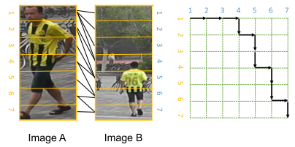
\includegraphics[width=\linewidth,keepaspectratio]{data/chapter-1/placeholder.png}
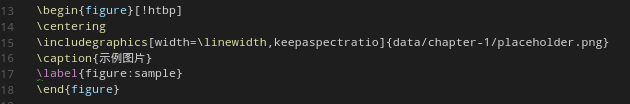
\includegraphics[width=\linewidth,keepaspectratio]{fig/2018-03-29-21-41-37.png}
\caption{示例图片}
\label{figure:sample}
\end{figure}

\section{本文结构安排}

如表~\ref{table:sample}

\begin{table}[!htbp]
\caption{示例表格}
\label{table:sample}
\centering
\begin{tabular}{|c|c|}
\hline
键 & 值 \\
\hline
键 1 & 值 1 \\
\hline
\end{tabular}
\end{table}

	\cleardoublepage
	\chapter{基于**的网络}

\section{第一节}

\section{本章小结}



	\cleardoublepage
	% !TeX root = ../main.tex

\chapter{基于**的网络}

\section{第一节}

\section{本章小结}



	\cleardoublepage
	% !TeX root = ../main.tex

\chapter{基于**的网络}

\section{第一节}

\section{本章小结}



	\cleardoublepage
  % !TeX root = ../main.tex

\chapter{结论与展望}

\section{第一节}

\section{本章小结}



  \cleardoublepage
  
	\renewcommand{\thechapter}{}
	\include{data/bibliography}
	\cleardoublepage

	% \include{data/acknowledgment}
	% \cleardoublepage
}

{
	\backmatter

	\pagestyle{empty}

	% \include{data/assignment}
	% \cleardoublepage

	% \include{data/assessment}
	% \cleardoublepage
}

\end{document}
